%http://www.cse.chalmers.se/edu/course/TDA231/mlsli11.pdf
K-nearest neighbors (KNN) algorithm is one of the simplest machine learning
algorithms. The classification performed by KNN works as follows: Fix some
number $k$. For any new $x \in X$, take the most common classification value among
the $k$ training examples in $D$ closest to $x$\cite{ml_2011}.

Even though the KNN algorithm
seems extraordinary simple there are some things that one must take in
consideration. First of all what is nearest? There is of course a natural
distance function in a geometrical space but a proper definition in parameter
space is not obvious. As it turn out a distance function can be defined in a lot
of ways. The given attributes are overall very different in reality.
One may may multiply each attribute variable by arbitrary factors or in other
words stretch the coordinate axes arbitrary and independent. It is very easy to
find examples when doing so will result in very different outcomes of the classifications.
Even further irrelevant attributes may change the classification even though they
shouldn't do so. This phenomena is called \emph{curse of dimensionality}. One
can try to find good stretch factors by performing cross validation.
One takes a vector of stretch factors that
minimizes the classification errors on a valid set. The back side is that
this will require a lot of test vectors\cite{ml_2011}.

An other problem is the computation complexity. KNN is sad to have a lazy
learning method. In other words it does output hypotheses in explicit form.
Instead a lot of computational steps are required for the classification\cite{ml_2011}.

A further issue is to find a suitable $k$. A great choose of $k$ various
depending on many circumstances. A keystone is that if the training set is large
it's important get rid of noise in the data hence increase $k$. On the other
hand a big $k$ requires more calculation. There are however also other more
complex ways for reducing noise \cite{ml_2011}.
%https://dl.dropbox.com/u/5139428/ml-course/Classification1.pdf
\begin{center}
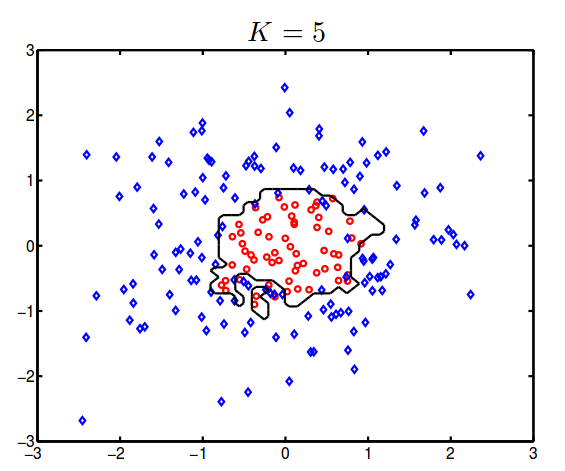
\includegraphics[scale=0.5]{fig/KNN.png}
\end{center}
